\subsubsection{12.11.2015}
\textit{\textbf{Time frame:}} 17:00-21:30 \newline
Today it was created the carriage. There were applied 7 cm standard wheels with gear ratio 2:1 (speed about $2 \times 7 \times 2 \times Pi = 88$cm/sec). Next motors were connected to motor controllers and an NXT brick (as we didn't have new control system) and it was realised a simple program to test the wheel base. Source code is available in the section "specifications for programs".
The prototype had no problem with movement on the field. However, it's clearance was too narrow and it couldn't climb to the inclined plane. So, it was decided to rebuild wheel base with 10 cm wheels.
It was also created the prototype of the gripper for debris.

\begin{figure}[H]
	\begin{minipage}[h]{0.37\linewidth}
		\center{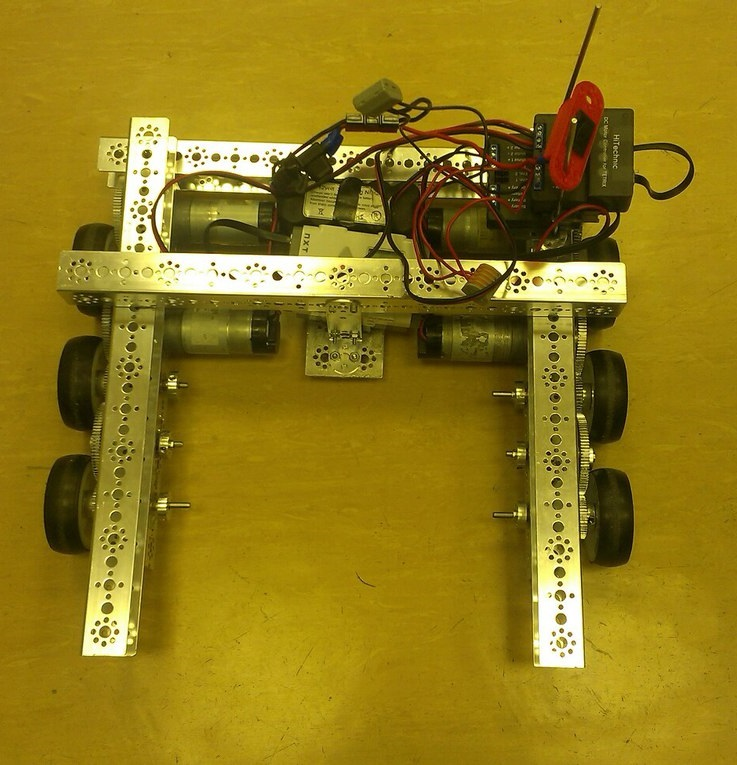
\includegraphics[scale=0.25]{3Engineering/5Team_meetings/days_of_meetings/2015.11.12/images/01}}
		\caption{Prototype of the wheel base}
	\end{minipage}
	\hfill
	\begin{minipage}[h]{0.58\linewidth}
		\center{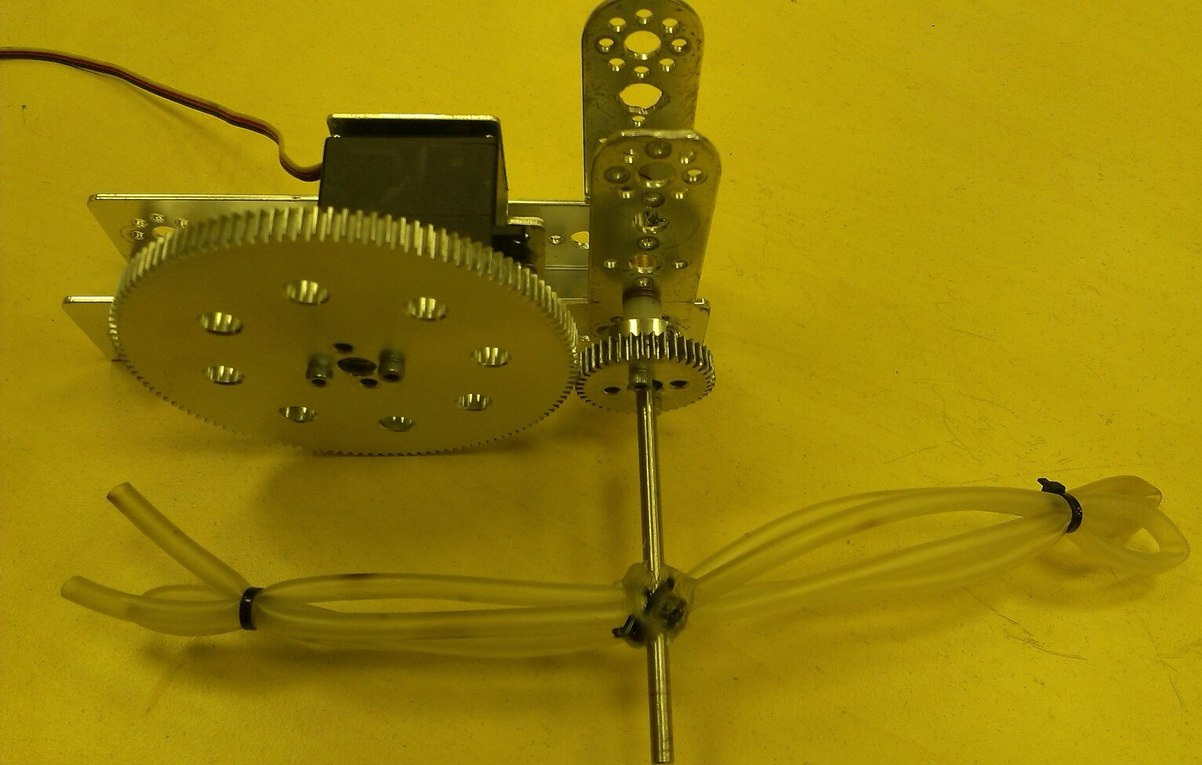
\includegraphics[scale=0.25]{3Engineering/5Team_meetings/days_of_meetings/2015.11.12/images/02}}
		\caption{Prototype of the gripper}
	\end{minipage}
\end{figure}
